\documentclass[letterpaper,11pt]{article}
% Soporte para los acentos.
\usepackage[utf8]{inputenc}
\usepackage[T1]{fontenc}
% Idioma español.
\usepackage[spanish,mexico, es-tabla]{babel}
% Soporte de símbolos adicionales (matemáticas)
\usepackage{multirow}
\usepackage{amsmath}
\usepackage{amssymb}
\usepackage{amsthm}
\usepackage{amsfonts}
\usepackage{latexsym}
\usepackage{enumerate}
\usepackage{ragged2e}
\usepackage{mathtools}
\usepackage{float}
% Soporte para referencias y citas
\usepackage{hyperref}
% Soporte para imágenes.
\usepackage{graphicx}
% Modificamos los márgenes del documento.
\usepackage[lmargin=2cm,rmargin=2cm,top=2cm,bottom=2cm]{geometry}

\title{Fundamentos de Bases de Datos \\
       Tarea 02. Modelo Entidad - Relación}

\author{Teresa Becerril Torres
        $\#$ de cuenta: $315045132$ \\
        Miguel Ángel Torres Sánchez
        $\#$ de cuenta: $315300442$ \\
        Nicole Romina Traschikoff García
        $\#$ de cuenta: $315164482$ \\
        Tania Michelle Rubí Rojas
        $\#$ de cuenta: $315121719$}

\date{06 de septiembre del 2019}
\begin{document}
\maketitle

\section{Repaso de conceptos generales}
\begin{itemize}
    \item[i.] Un conjunto de \textbf{entidades débiles} siempre se puede
    convertir en un conjunto de \textbf{entidades fuertes} añadiéndoles a sus
    atributos la \textbf{llave primaria} del conjunto de entidades fuertes a
    las que está asociado. Describe qué tipo de redundancia resultaría si se
    realizara dicha conversión.

    \textsc{Solución:} Tendríamos redundancia porque en los dos conjuntos vamos
    a tener información duplicada a causa de estar añadiéndo las llaves
    primarias.

    \item[ii.] Responde a las siguientes cuestiones, deberpas indicar
    \textbf{si son posibles o no}, justificando tu respuesta. Cuando no sea
    posible deberás indicar alguna recomendación al respecto.

    ¿Un \textbf{atributo compuesto} puede ser llave? \\
	\textsc{Solución:} Sí puede ser llave pero solo cuando todos sus componentes lo son, así cada entidad puede ser identificada por un conjunto de llaves.\\
    ¿Un \textbf{atributo multivaluado} puede ser \textbf{llave}?\\
	\textsc{Solución:} Sí puede ser, porque la entidad a la que corresponda ese atributo puede ser identificada por más de una sola llave.\\
    ¿Un \textbf{atributo derivado} puede ser \textbf{llave}?\\
	\textsc{Solución:} Sí puede serlo si la forma en que se calcula o deriva devuelva un valor único del dominio del atributo, así todas llaves identifican a una entidad.\\
    ¿Un \textbf{atributo multivaluado} puede ser \textbf{compuesto}?\\
	\textsc{Solución:} No puede serlo, podría ocurruri redundancia si dos entidades tienen los mismos valores del dominio del atributo. Sería recomendable transformar el atributo en una nueva entidad con sus respectivos atributos y relacionar las entidades incluyendo una nueva relación total de muchos a muchos.\\
    ¿Un \textbf{atributo multivaluado} puede ser \textbf{derivado}?\\
	\textsc{Solución:} No puede serlo pues el derivado se obtiene con ciertos parámetros y en un principio con los mismos parámetros deberían obtenerse los mismos resultados, por lo tanto no es posible tener varios valores para un atributo derivado. Sería recomendable modificar el modelo para no necesitar hacer muchos cálculos para un mismo atributo o hacer nuevos atributos derivados para cada cosa que se necesita calcular.\\
    ¿Qué implicaría la existencia de una \textbf{entidad} cuyos atributos sean \textbf{todos derivados}? \\
	\textsc{Solución:} Implicaría que la entidad depende completamente de otras entidades y sus relaciones con ellas.


<<<<<<< HEAD
    \item[iii.] Explica el concepto de \text{agregación} en el
=======
    \item[iii.] Explica el concepto de \text{agregación} en el 
>>>>>>> 3b551f4e67b2bb6384589411aff7d81a3c1fd5cf
    \textbf{modelo E/R} y proporciona un par de ejemplos.

    La agregación es una abstracción mediante la cual las relaciones
    son tratadas como un conjunto de entidades de alto nivel. Se
    representa como un conjunto de entidades y relaciones encerradas
    en un recuadro.

    \begin{itemize}
        \item  \textbf{Ejemplo 1:}

               Queremos registrar en una base de datos información acerca
               de los cursos que se enseñan en una escuela donde cada
               curso puede ser enseñado por muchos profesores y en él
               se pueden inscribir muchos alumnos.

               \begin{figure}[h]
                \centering
                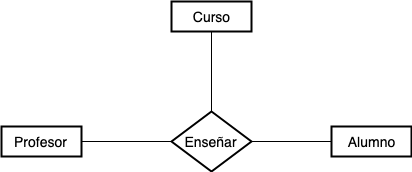
\includegraphics[scale=0.6]{./imagenes/Ejemplo1.jpg}
                \end{figure}

               Y queremos tener un reporte de evaluación del
               progreso del curso después de cada periodo de examenes,
               por lo que necesitamos saber los alumnos y profesores
               involucrados en el curso, también necesitamos saber
               la secretaria que realizo el reporte.

               \begin{figure}[H]
                \centering
                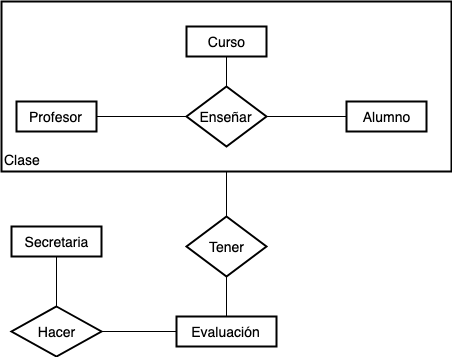
\includegraphics[scale=0.6]{./imagenes/Ejemplo1a.jpg}
                \end{figure}

               Nos conviene utilizar agregación ya que nos
               permite relacionar evaluación con la entidad
               secretaria y la entidad creada por la agregación (clase)
               sin crear una relación rendudante o compleja con la que
               no podríamos relacionar directamente secretaria.



            \item \textbf{Ejemplo 2:}

            Queremos registrar en una base de datos información acerca
            de máquinas que se utilizan en una fabrica donde cada máquina
            puede ser ocupada por varios trabajadores.

            \begin{figure}[h]
             \centering
             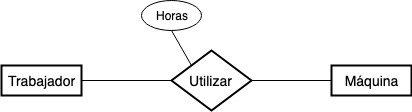
\includegraphics[scale=0.6]{./imagenes/Ejemplo2.jpg}
             \end{figure}

            Queremos tener un balance cada tres meses del estado de las
            máquinas por lo que se necesita saber los trabajadores que
            las utilizan y tener la información del contador que lo realizo.

            \begin{figure}[H]
                \centering
                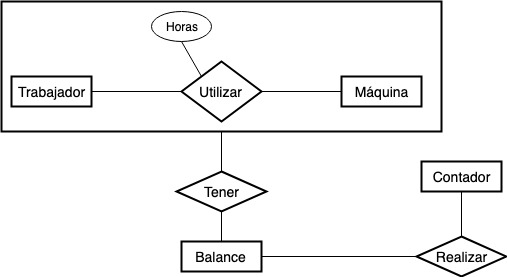
\includegraphics[scale=0.6]{./imagenes/Ejemplo2a.jpg}
                \end{figure}

            Utilizando agregación nos permite relacionar  con la entidad
            contador y la entidad creada por la agregación sin crear
            relaciones rendudantes o complejas.

        \end{itemize}

    \item[iv.] Diseña una base de datos que represete los conceptos revisados
    para crear un \textbf{diagrama E/R} (no consideres el Modelo E/R extendido).
          \begin{figure}[h]
           \centering
           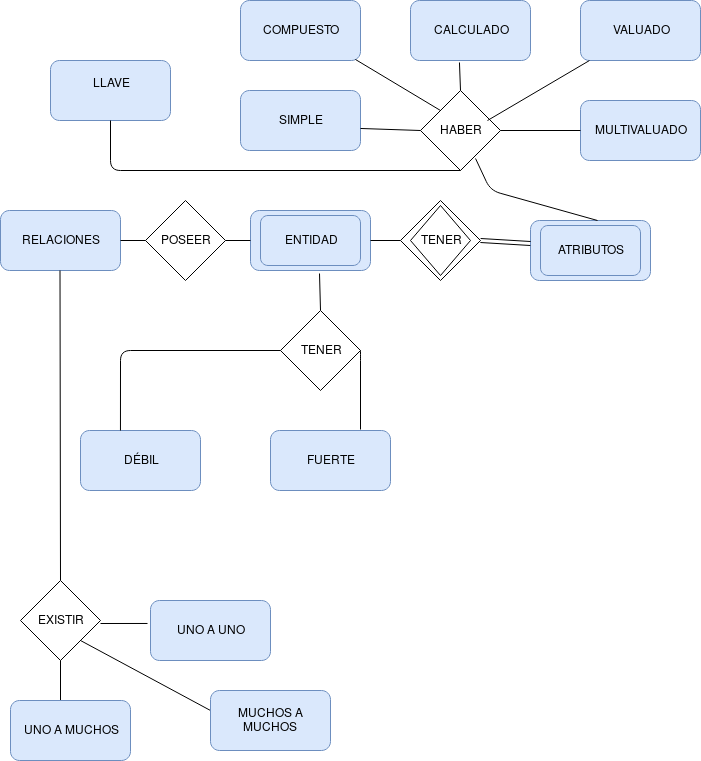
\includegraphics[scale=0.6]{./imagenes/iv.png}
           \end{figure}

\end{itemize}

\section{Modelo Entidad/Relación}

\begin{itemize}
    \item[a.] \textbf{Empresa de envíos} \\
    Una \textbf{empresa de envíos} desea modernizar su administración de envíos,
    para la cual se desea diseñar una \text{base de datos} a partir de las
    siguientes restricciones del negocio:

    \begin{itemize}
        \item[i.] La empresa cuenta con una serie de \text{vehículos para transporte},
        de los cuales de desea almacenar su \textbf{número de motor, marca, modelo,
        tipo, descrpción, fecha de compra y precio de compra}. Cada vehículo estará
        a cargo de un \textbf{supervisor} para la realización de su mantenimiento.
        Todo transporte debe tener asignado un sólo supervisor y cada supervisor
        estará a carga de al menos un vehículo.

        \item[ii.] Los vehículos son de \textbf{tres tipos: motos, van y aviones}.
        de las \text{motos} interesa almacenar su \textbf{cilindraje}, de las
        \textbf{van} su \textbf{capacidad} y de los \textbf{aviones} del tipo de
        \textbf{fuselaje}. De los \textbf{supervisores} interesa conocer el
        \textbf{RFC, nombre completo, dirección, teléfono y transportes a su cargo}.

        \item[iii.] La empresa maneja \textbf{dos tamaños básicos} para las
        mercancías: \textbf{sobres y paquetes}. De los \textbf{sobres} interesa
        conocer el \textbf{peso} y de los \textbf{paquetes} las \textbf{dimensiones}.
        En los envíos, los \textbf{sobres se asignan a una moto} para su
        transporte y no puede haber sobres sin asignar a motos; una moto puede tener
        asignados varios sobres o ninguno. Si la mercancía es \textbf{un paquete},
        se \textbf{asignará una van} con las mismas restricciones que se tienen los
        sobres y las motos.

        \item[iv.] De las \textbf{mercancías enviadas} se almacenará el
        \textbf{código, la descripción, el precio del envío, si están aseguradas} y
        si son \textbf{al interior de la república}. Si las mercancías son al
        \textbf{interior de la república}, entonces de les \textbf{asignará
        adicionalmente un avión}. No puede haber mercancías que se envíen al interior
        de la república que no tengan asignado un avión.

        Un avión puede tener asignadas varias o ninguna mercancía de larga distancia.
        Una mercancía de larga distancia debe tener asignada su correspondiente moto
        o van para llevarla empresa/aereopuerto/destino final.

        \item[v.] Los \textbf{clientes} de la empresa de envíos son empresas o
        particulares, de estos clientes interesa almacenar el \textbf{código de
        cliente, la fecha y el total facturado} a dicho cliente. Si el
        \textbf{cliente es un particular} se almacenará su \textbf{RFC, nombre
        completo, dirección y teléfonos}. Si el cliente es una \textbf{empresa}, se
        almacenará el \textbf{RFC, razón social, dirección, teléfonos y correo
        eléctronico}.

        \item[vi.] De los \textbf{envíos de mercancías} hay que almacenar el
        \textbf{cliente que realiza el envío, el destinatario, la mercancía
        enviada y la fecha de envío}. Los clientes pueden encargar el envío de
        sus mercancías a dos tipos de destinatarios: \textbf{empresas o
        particulares}. Si el envío es a una empresa se debe enviar al menos una
        mercancía. Si el envío tiene como destino un particular, se cobrará el
        almacenaje que consiste en el $4 \%$ del precio original del envío. En
        cualquiera de los dos casos se cobrará un $1 \%$ más por cada vez que no
        se ha conseguido realizar la entrega. Interesa, entonces almacenar el
        número de intentos de entrega de una mercancía a un particular y se
        deben almacenar todos los envíos encargados por el cliente.
    \end{itemize}

    \item[b.] \textbf{Sistema de información geográfica}
    La \textbf{Secretaría del Medio Ambiente y Recursos Naturales (SEMARNAT)}
    desea crear un \textbf{SIG} (Sistema de Información Geográfica) para acceso
    público a través de internet. El sistema ofrecerá la siguiente información:

    \begin{itemize}
        \item Datos referentes a \textbf{ríos, sistemas montañosos, montañas y
              municipios} donde se localizan.
        \item De los \textbf{ríos} se almacenará un identifacador del río, nombre,
              descripción y longitud total. Para cada río, además, se almacenarán
              los municipios que atraviesa la longitud del tramo del río para cada
              municipio bañado.
        \item De los \textbf{municipios} se almacenará un identificador para
              el municipi, nombre, y número de habitantes.
        \item Los \textbf{ríos} pueden ser afluentes de otros ríos, si es el caso,
              se desea conocer a cuál río alimentan y el municipio en el que se unen
              al río del que son afluentes.
        \item En cuanto a los \textbf{sistemas montañosos} se almacenará un código,
              el nombre, la orientación (norte, sur, este, oeste), la longitud, la
              altura máxima y los municipios que ocupa. Los sistemas están formados
              por \textbf{montañas} de los que se almacena un código, un nombre,
              descripción y altura. Se debe considerar que una montaña solo
              pertenecerá a un sistema montañoso. Se requiere también almacenar
              el municipio o municipios en lo que se encuentra, ya que hay casos
              en los que una montaña es compartida por varios municipios.
        \item Las \textbf{montañas} además pueden tener un \textbf{origen volcánico}
              o de \textbf{plegamiento}. En el caso de que su origen sea volcánico,
              se desea almacenar el tipo de volcán y si es de plagamiento, se desea
              almacenará el periodo geológico de dicho plegamiento.
        \item \textbf{Algunos ríos} y \textbf{montañas} son elementos geológicos
              \textbf{monitoreados por satélite}. De dichos elementos se desea
              alamcenar la fecha en la que se comienza a monitorear y el satélite
              que realiza el seguimiento. Un satélite puede monitorear varios
              elementos. De los satélites se desea almacenar su identificador,
              nombre y descripción
    \end{itemize}
\end{itemize}

\section{Ingeniería inversa}
Una \textbf{compañía celular} requiere una base de datos para realizar un
seguimiento de sus \textbf{clientes}, sus \textbf{planes de suscripción} y
\textbf{los teléfonos móviles} que están utilizando. El diagrama \textbf{E/R}
de la siguiente figura muestra entidades de interés para la compañía y las
relaciones entre ellas. Tomando como base el esquema proporcionado, responde a
las siguientes preguntas justificando tu respuesta. Para cada pregunta,
identificar el o los elementos en el diagrama $E/R$ que utilizaste para tu
respuesta. En caso de que alguna pregunta no se cumpla en el diagrama actual,
indica las modificaciones que deberían hacerse para que se permita dicho
comportamiento.

\begin{figure}[h]
    \centering
    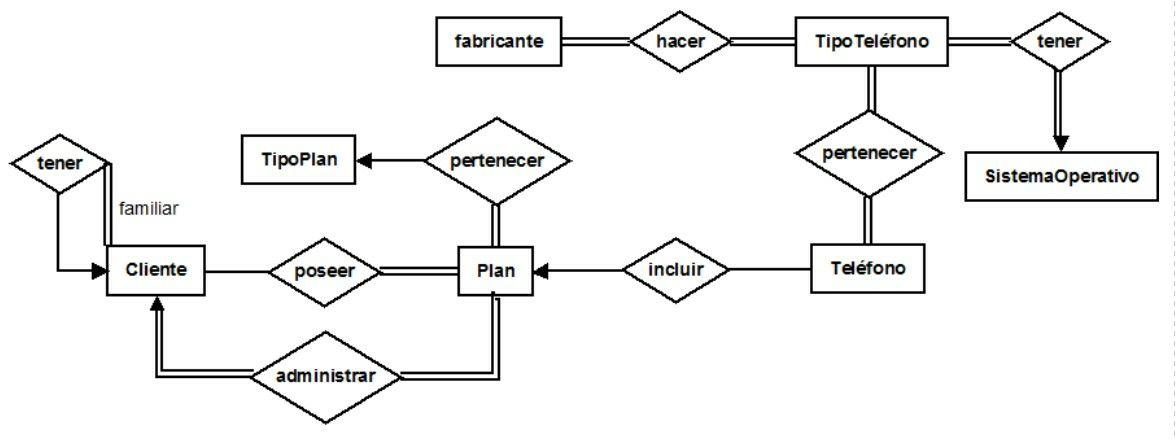
\includegraphics[scale=0.4]{./imagenes/modelo.jpg}
\end{figure}

\begin{itemize}
    % Ejercicio 1.
    \item ¿Un cliente puede tener un número ilimitado de planes?

<<<<<<< HEAD
    \textsc{Solución:} Sí. La zona rosa nos dice que hay una relación $1:m$
    donde \textit{un cliente tiene varios tipos de planes} ya que
    \textit{Un plan pertence a un tipo de plan}. Entonces, si el
=======
    \textsc{Solución:} Sí. La zona rosa nos dice que hay una relación $1:m$ 
    donde \textit{un cliente tiene varios tipos de planes} ya que 
    \textit{Un plan pertence a un tipo de plan}. Entonces, si el 
>>>>>>> 3b551f4e67b2bb6384589411aff7d81a3c1fd5cf
    cliente lo desea, puede llegar a tener una infinidad de planes.

    \begin{figure}[h]
        \centering
        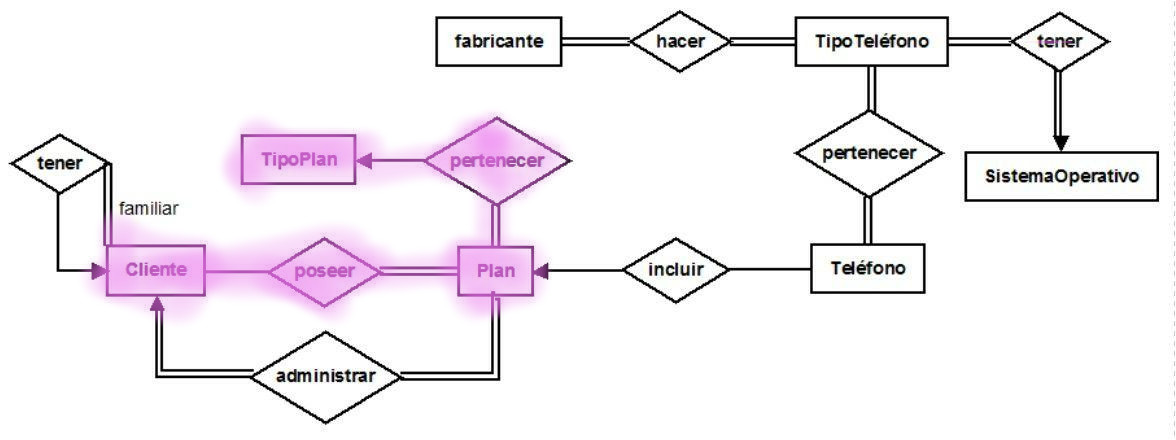
\includegraphics[scale=0.4]{./imagenes/modelo1.jpg}
    \end{figure}

    % Ejercicio 2.
    \item ¿Un cliente puede existir sin un plan?

<<<<<<< HEAD
    \textsc{Solución:} Sí. La relación \textit{poseer} relaciona las entidades \textit{Cliente} y \textit{Plan} donde la participación de la entidad \textit{Cliente} es parcial, por lo tanto puede existir algún cliente que no posee un plan.
=======
    \textsc{Solución:} Sí. La relación \textit{poseer} relaciona las entidades \textit{Cliente} y \textit{Plan} donde la participación de la entidad \textit{Cliente} es parcial, por lo tanto puede existir algún cliente que no posee un plan. 
>>>>>>> 3b551f4e67b2bb6384589411aff7d81a3c1fd5cf

    % Ejercicio 3.
    \item ¿Es posible crear un plan sin saber quién es el cliente?
    
    No debido a que la participación de plan es total en las relaciones \textit{poseer} 
    y \textit{administrar} por lo que \textit{cada plan debe relacionarse con al menos 
    un cliente}. 
    \begin{figure}[H]
        \centering
        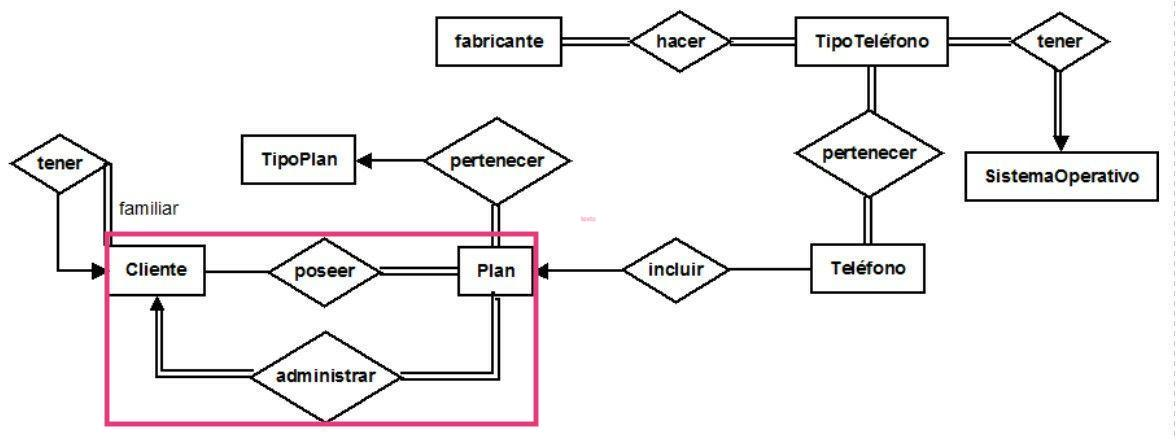
\includegraphics[scale=0.4]{./imagenes/modelo3a.jpg}
    \end{figure}
    Para que sea posible crear un plan si saber quién es el cliente la participación
    de plan debería se parcial.
    \begin{figure}[H]
        \centering
        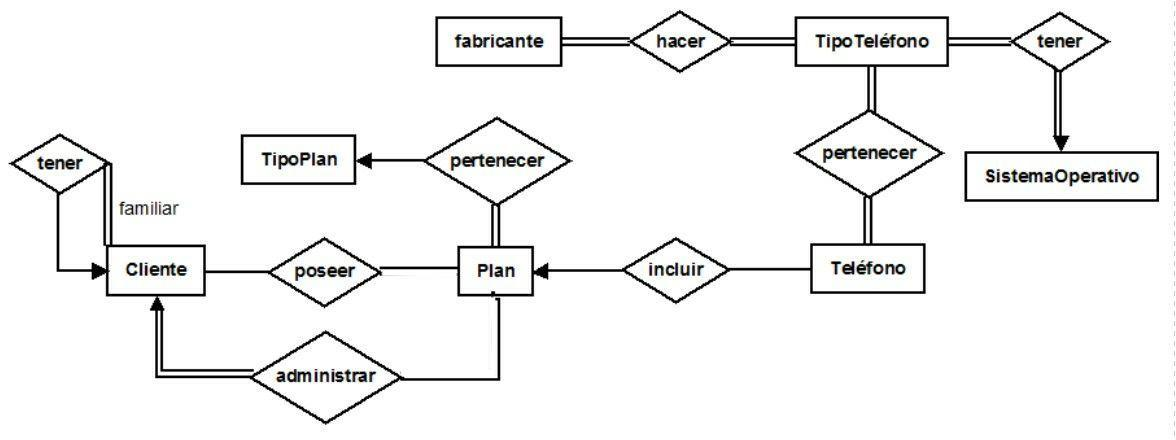
\includegraphics[scale=0.4]{./imagenes/modelo3b.jpg}
    \end{figure}

    No debido a que la participación de plan es total en las relaciones \textit{poseer}
    y \textit{administrar} por lo que \textit{cada plan debe relacionarse con al menos
    un cliente}.
    \begin{figure}[H]
        \centering
        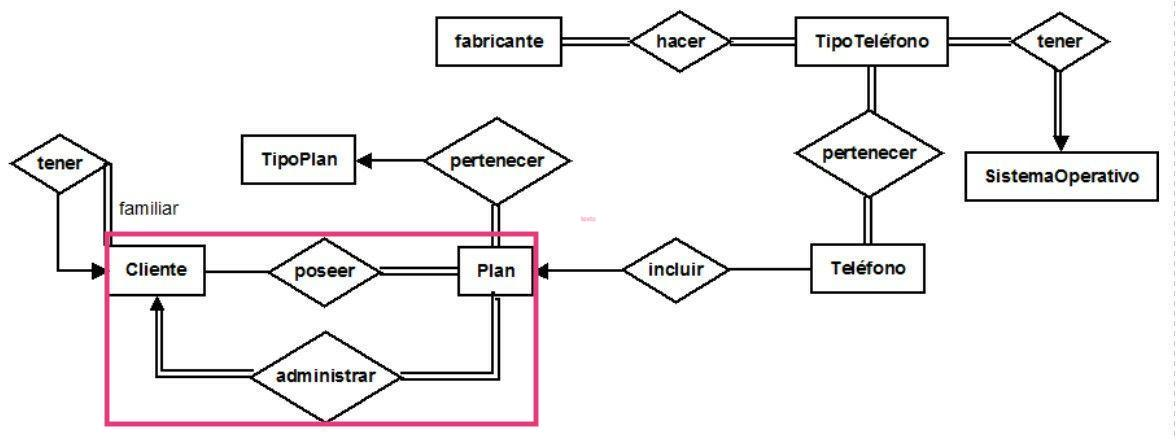
\includegraphics[scale=0.4]{./imagenes/modelo3a.jpg}
    \end{figure}
    Para que sea posible crear un plan si saber quién es el cliente la participación
    de plan debería se parcial.
    \begin{figure}[H]
        \centering
        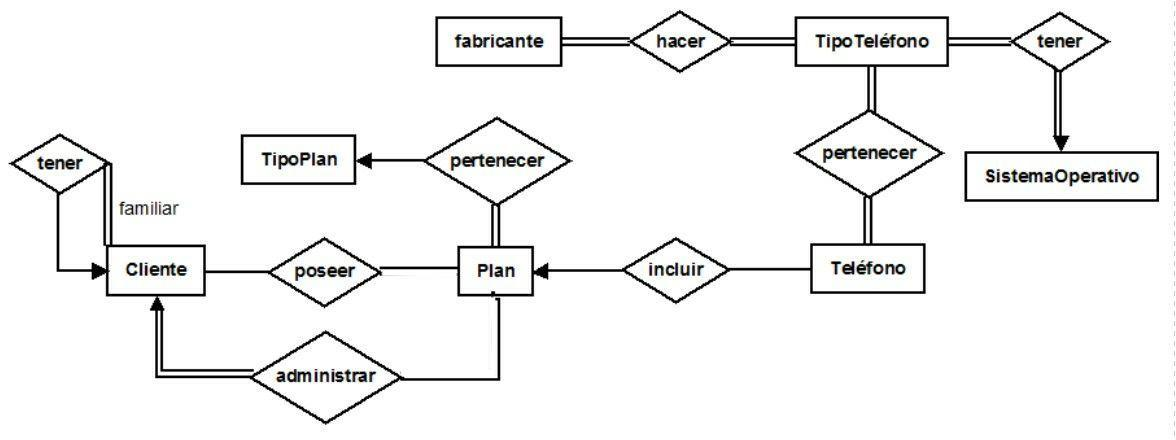
\includegraphics[scale=0.4]{./imagenes/modelo3b.jpg}
    \end{figure}

    % Ejercicio 4.
    \item ¿El operador quiere limitar los tipos de dispositivos que se pueden
    vincular a un tipo de plan específico?

    % Ejercicio 5.
    \item ¿Es posible mantener los datos relativos a un teléfono sin conectarlo
    a un plan?

    \textsc{Solución:}

    % Ejercicio 6.
    \item ¿Puede un teléfono puede asociar a varios planes?

    \textsc{Solución:} No. La entidad \textit{Teléfono} y la entidad \textit{Plan} se asocian con la relación \textit{Incluir} que es una relación uno a muchos, por lo tanto un teléfono está asociado a lo más a un solo plan, pero un plan sí puede estar asociado a muchos teléfonos o a ninguno. Cambiar la cardinalidad de la relación \textit{Incluir} a la de una relación muchos a muchos nos permitiría asociar un teléfono a más de un plan.
<<<<<<< HEAD

=======
    
>>>>>>> 3b551f4e67b2bb6384589411aff7d81a3c1fd5cf
    % Ejercicio 7.
    \item Supongamos que existe un tipo de teléfono que puede utilizar múltiples
    sistemas operativos. ¿Esta situación podría tener cabida dentro del modelo
    incluido en la figura?

<<<<<<< HEAD
    No, porque la relación \textit{tener} es $n:1$ donde \textit{varios tipos de
=======
    No, porque la relación \textit{tener} es $n:1$ donde \textit{varios tipos de 
>>>>>>> 3b551f4e67b2bb6384589411aff7d81a3c1fd5cf
    telefonos tienen solo un sistema operativo}

    \begin{figure}[H]
        \centering
        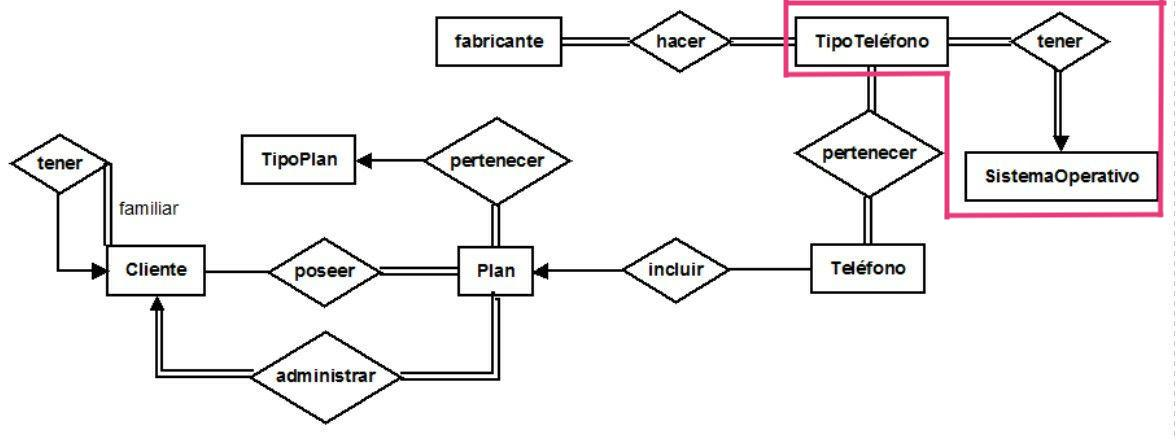
\includegraphics[scale=0.4]{./imagenes/modelo7a.jpg}
    \end{figure}

<<<<<<< HEAD
    Para que esto ocurra debemos cambiar la cardinalidad de la relación
=======
    Para que esto ocurra debemos cambiar la cardinalidad de la relación 
>>>>>>> 3b551f4e67b2bb6384589411aff7d81a3c1fd5cf
    \textit{tener} de $n:1$ a $n:m$.
    \begin{figure}[H]
        \centering
        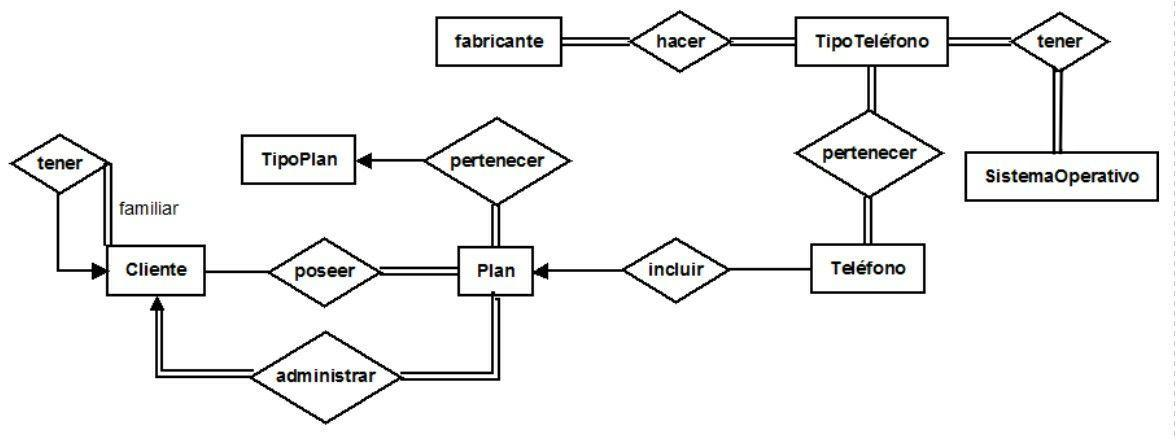
\includegraphics[scale=0.4]{./imagenes/modelo7b.jpg}
    \end{figure}

    % Ejercicio 8.
    \item ¿La empresa es capaz de realizar un seguimiento de un fabricante sin
    mantener información sobre sus teléfonos?

    % Ejercicio 9.
    \item ¿El mismo sistema operativo se puede utilizar en mútiples tipos de
    dispositivos?

    \textsc{Solución:} No. La parte azul del diagrama nos muestra que la
    relación es de uno a muchos, donde \textit{un teléfono tiene varios
    sistemas operativos} ya que \textit{Un tipo de teléfono tiene varios
    sistemas operativos}.

    \begin{figure}[H]
        \centering
        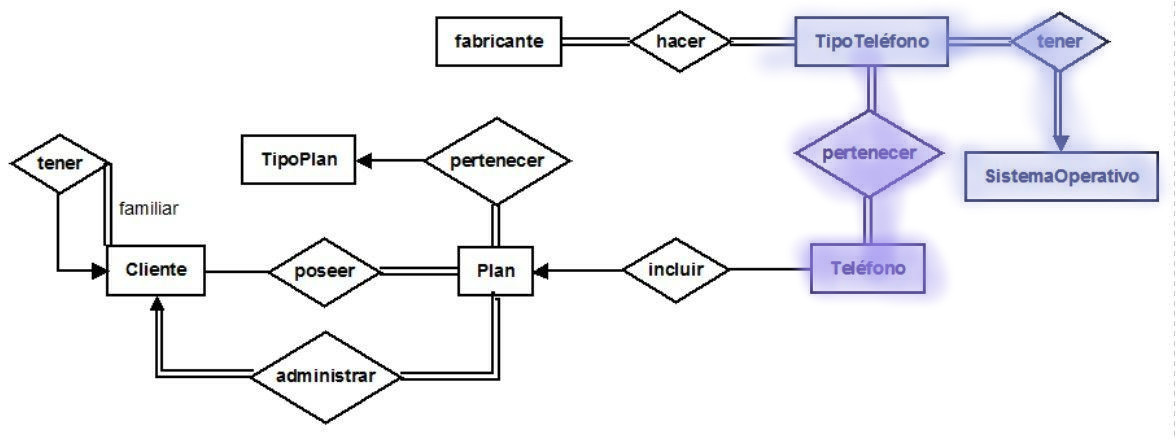
\includegraphics[scale=0.4]{./imagenes/modelo9.jpg}
    \end{figure}

    Para hacer la modificación, lo que tenemos que hacer es una relación $m:1$,
    donde \textit{el mismo sistema operativo utiliza varios tipos de teléfono}.
    Esto se representa de la forma

    \begin{figure}[H]
        \centering
        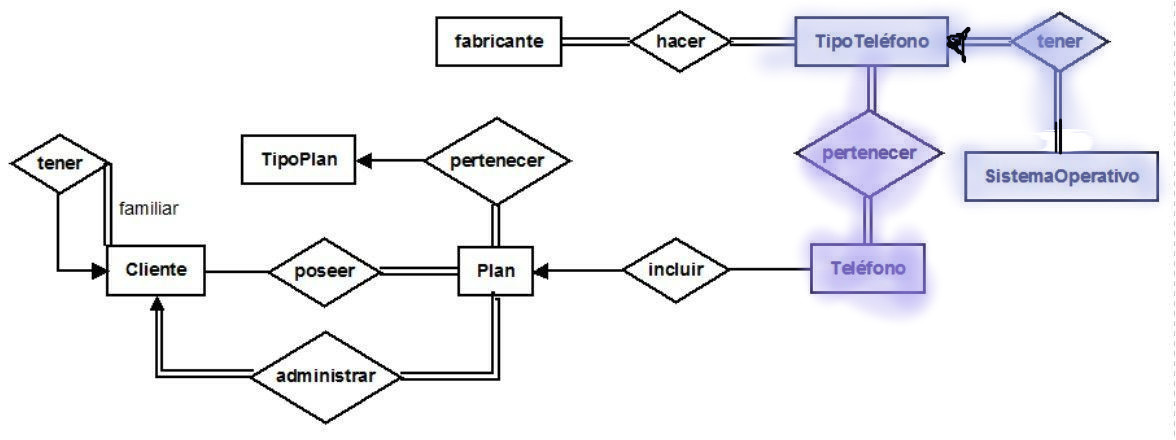
\includegraphics[scale=0.4]{./imagenes/modelo9i.jpg}
    \end{figure}

    % Ejercicio 10.
    \item Hay dos relaciones entre el Cliente y el Plan. Explicar en qué
    difieren.

    \textsc{Solución:} La relación \textit{poseer} nos permite asociar a todos los planes con algunos clientes, hay clientes que pueden no poseer un plan pero a todos los planes los posee un cliente, además un mismo cliente puede poseer varios planes y un mismo plan puede ser posesión de varios clientes.
La relación \textit{administrar} relaciona a todos los clientes con todos los planes, todos los planes son administrados por un solo cliente y todos los clientes pueden admnistrar varios planes.
<<<<<<< HEAD
La diferencia entre ambas relaciones está en su cardinalidad y la participación de las entidades \textit{Cliente} y \textit{Plan} en cada una.
=======
La diferencia entre ambas relaciones está en su cardinalidad y la participación de las entidades \textit{Cliente} y \textit{Plan} en cada una. 
>>>>>>> 3b551f4e67b2bb6384589411aff7d81a3c1fd5cf

    % Ejercicio 11.
    \item Caracterizar el grado y la cardinalidad de la relación que une al
    cliente a sí mismo. Explicar su significado.

<<<<<<< HEAD
    La relación \textit{tener} es de grado 1 (relación reflexiva) y su
    cardinalidad es $1:n$ (uno a muchos).
=======
    La relación \textit{tener} es de grado 1 (relación reflexiva) y su 
    cardinalidad es $1:n$ (uno a muchos). 
>>>>>>> 3b551f4e67b2bb6384589411aff7d81a3c1fd5cf

    \begin{figure}[H]
        \centering
        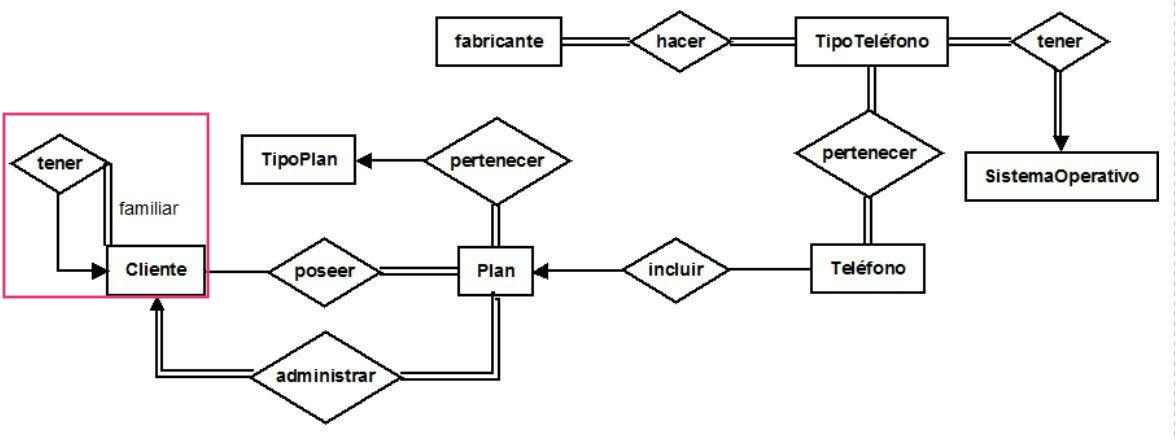
\includegraphics[scale=0.4]{./imagenes/modelo11.jpg}
    \end{figure}

    Significa que un cliente puede tener varios clientes familiares.
    % Ejercicio 12.
    \item ¿Es posible vincular un teléfono a un cliente específico en un plan
    con múltiples clientes?

    % Ejercicio 13.
    \item ¿Puede la compañía rastrear un teléfono sin identificar sus sistema
    operativo?

\end{itemize}

\end{document}
